\subsubsection{Umsetzung der theoretischen Modelle in der Simulationssoftware}
\label{chap:Umsetzung der theoretischen Modelle in der Simulationssoftware}

Ein erster, naiver Ansatz zur Implementierung des \ac{ep} beinhaltet die Aufteilung des zweiphasigen Lernprozesses in zeitlich getrennte Abläufe. Damit wird ein einziges \ac{hnn} benötigt, um Inferenz mit \(\beta=0\) und \(\beta>0\) durchzuführen.

Die Integratoren zur Repräsentation der Gewichte müssen dafür zurücksetzbar sein, was in Simulink durch den Parameter "`External reset"' am Integrator-Block möglich ist. Auf einem analogen Computer kann dies durch den Wechsel der Modi "`IC"' bzw. "`OP"' erfolgen (vgl. Kapitel \ref{chap:Typische Komponenten und Bauweisen analoger Computer}). Der "`Pulse Generator"'-Block aus Simulink kann so konfiguriert werden, dass er innerhalb einer gesetzten Periodendauer zwischen den Werten \(0\) und \(1\) wechselt und somit die Zeitsteuerung abbildet. Dafür muss für die praktische Umsetzung ein externes Bauteil zum Einsatz kommen, da, basierend auf den in Kapitel \ref{chap:Typische Komponenten und Bauweisen analoger Computer} genannten Plattformen, Pulsgeneratoren nicht auf analogen Computern bereitgestellt werden. Als weitere Komponente wird der Komparator benötigt, welcher anhand des Signals des Pulsgenerators die aktive Phase des Lernprozesses bestimmt und in Simulink als "`Switch"'-Block abgebildet wird. Dieser Block findet Anwendung am Lernparameter \(\beta\), am Zurücksetzen der Integratoren und als Schranke zur Weiterverarbeitung der Zustände des Netzwerks.

Durch die Zeitsteuerung des Lernprozesses ist zu jeder Zeit nur eine der beiden Phasen aktiv. Aus diesem Grund müssen die Zustände des Netzwerks nach der freien Phase zwischengespeichert werden, um sie nach Abschluss der festen Phase weiterverarbeiten zu können. Im hier vorgestellten Modell (siehe \ref{app:Umsetzung des Equilibrium-Propagation in Simulink}), ist dieser Mechanismus über den "`Memory"'-Block in Simulink zusammen mit einer Rückkopplung seiner Ausgabe zum vorgeschalteten Komparator gelöst. Die damit erzeugte Ausgabe aus Abbildung \ref{fig:Output EqProp 1} zeigt die Wirksamkeit der Zeitsteuerung, da alle zwanzig Sekunden für beide Phasen ein Fixpunkt des Netzwerks gefunden wird. Aus den Graphen wird aber auch deutlich, dass die Simulation durch die Nutzung der "`Memory"'-Blöcke mit diskreten Werten arbeitet, wodurch sich dieser Ansatz nicht für die Umsetzung auf analogen Computern eignet. Die Dokumentation des \ac{that} beschreibt zwar den "`HALT"'-Modus, wodurch die Integratoren ihren letzten Wert behalten und damit scheinbar für diesen Prozess genutzt werden können, dieser Modus soll aber laut der Dokumentation primär für Diagnostik und Fehlerbehebung genutzt werden \ua aus dem Grund, dass die gespeicherten Werte über Zeit an Genauigkeit verlieren (\cite[vgl.]{website:anabrid:that-docs}).

\begin{figure}[h]
  \caption{Ausgabe des zweiphasigen Lernprozesses des \ac{ep} im ersten vorgestellten Ansatz}
  \centering
  \begin{subfigure}[b]{0.5\textwidth}
    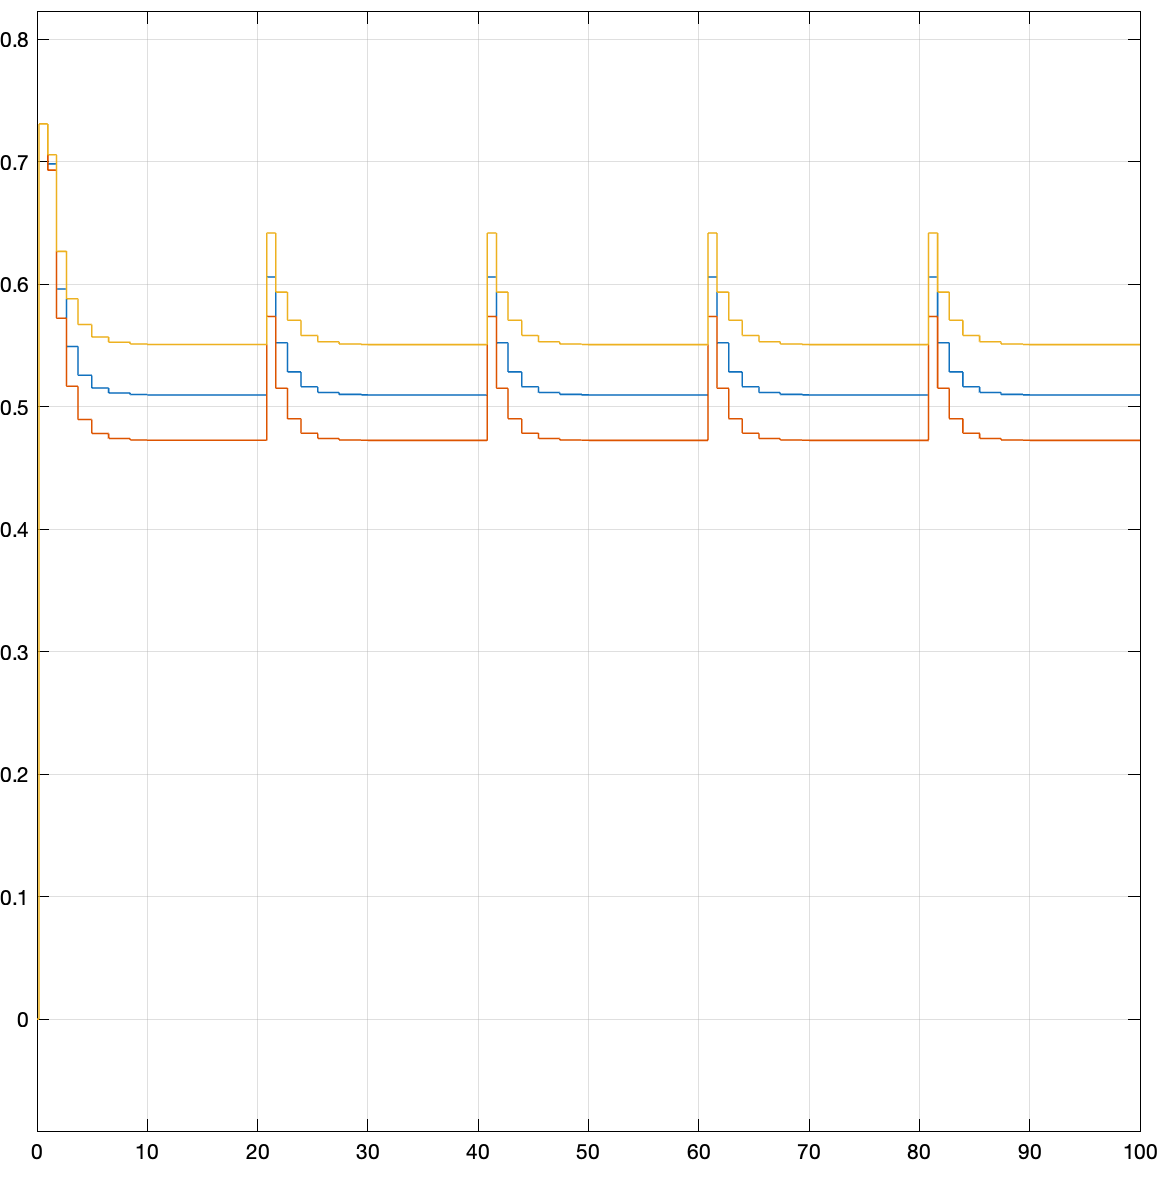
\includegraphics[width=\textwidth]{abbildungen/eqprop_discrete_free_output.png}
    \caption{Freie Phase}
  \end{subfigure}%
  \hfill
  \begin{subfigure}[b]{0.5\textwidth}
    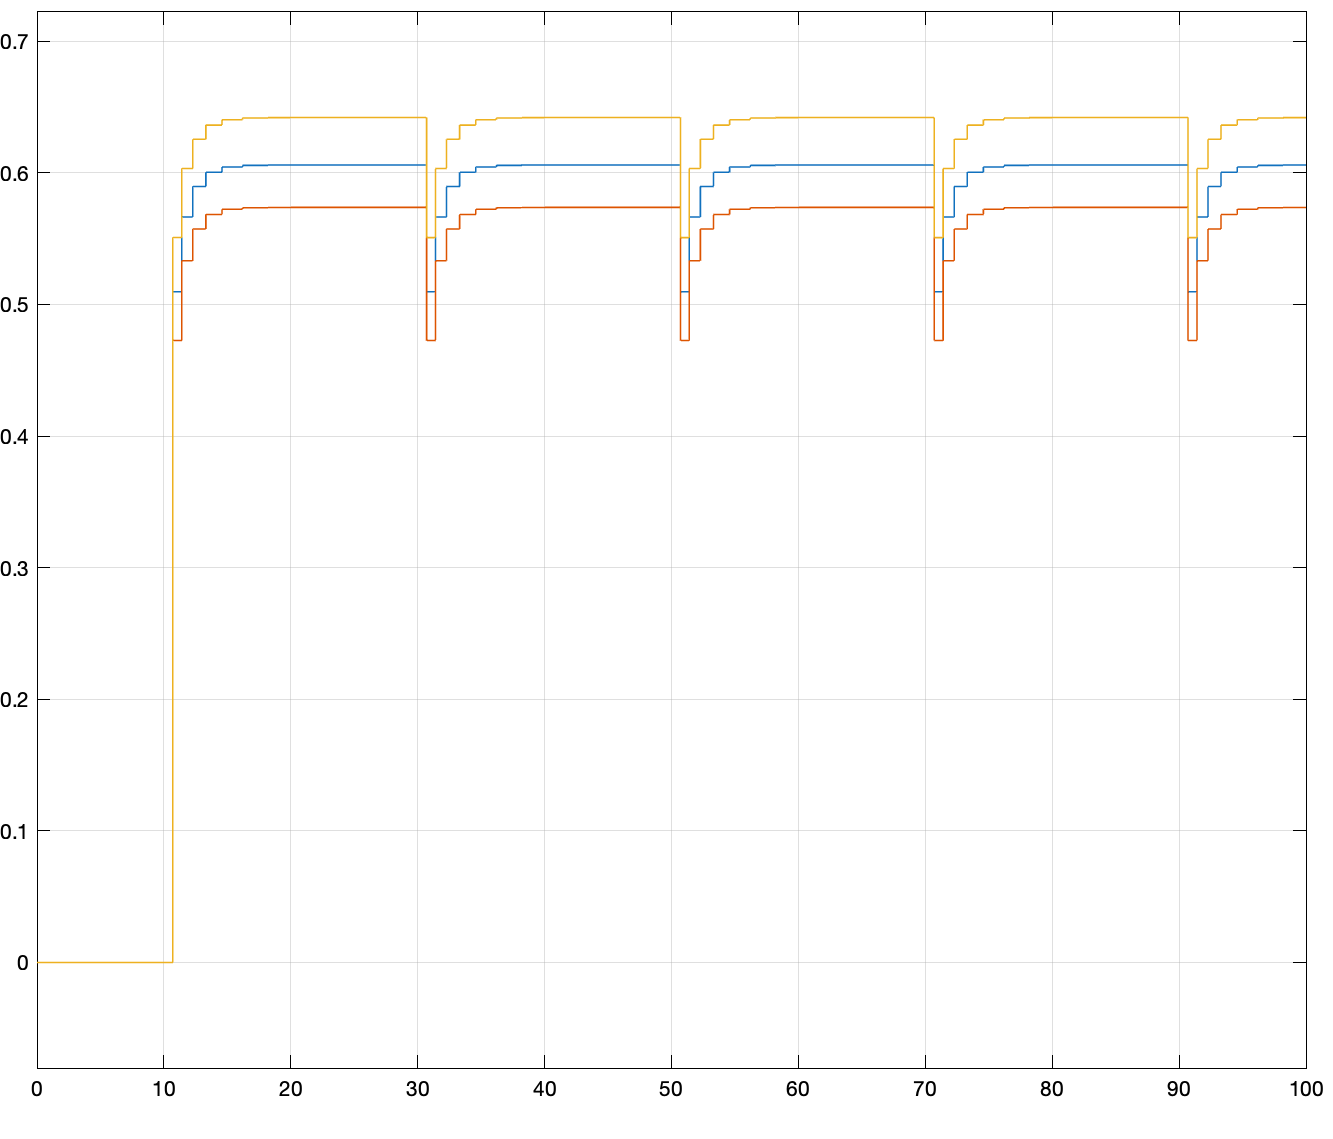
\includegraphics[width=\textwidth]{abbildungen/eqprop_discrete_clamped_output.png}
    \caption{Feste Phase}
  \end{subfigure}
  \\
  Quelle: Eigene Darstellung
  \label{fig:Output EqProp 1}
\end{figure}

In einer Arbeit von \citeauthor{Kendall2020} wurde bereits gezeigt, dass \ac{ep} in einer analogen Simulation in Zusammenarbeit mit herkömmlicher Software implementiert werden kann. \citeauthor{Kendall2020} stellte dafür einen Ansatz mithilfe der Simulationssoftware SPICE sowie Python vor, wobei innerhalb von SPICE das neuronale Netzwerk implementiert und damit die Fixpunkte der beiden Phasen gefunden wurden. Für die restlichen Bestandteile des Lernprozesses, wie die Berechnung der Fehlerfunktion oder die Anwendung der Lernregel, kam Python als digitaler Co-Prozessor zum Einsatz (\cite[vgl. S. 27]{Kendall2020}). Die Entwicklung eines hybriden Rechners ist aber nicht Teil dieser Arbeit, weshalb dieser Ansatz nicht weiter verfolgt wird.

Damit das \ac{ep} auf analoger Hardware realisierbar wird, muss eine kontinuierliche Lernregel aufgestellt werden. Einen Ansatz hierfür bietet das \citeyear{Ernoult2020} von \citeauthor{Ernoult2020} vorgestellte \ac{c-ep}. Diese Abwandlung des \ac{ep} bietet einerseits seine räumliche Lokalität, welche durch die Eigenschaft der Lernregel \(\Delta W_{ij}\), nur mit den beiden Zuständen \(u_{i}\) und \(u_{j}\) auszukommen, gegeben ist (siehe Kapitel \ref{chap:Theoretische Anwendung am Beispiel eines Hopfield-Netzwerks}). Zusätzlich arbeitet \ac{c-ep} lokal in Zeit, da der Zugriff auf das Ergebnis der freien Phase nach der festen Phase entfällt (\cite[vgl. S. 3 f.]{Ernoult2020}). Im \ac{c-ep} werden die Parameter \(\theta\) des Modells nicht durch eine Lernregel wie \(\Delta W\) aktualisiert, sondern ähnlich wie die Zustände des Modells, durch eine Dynamik beschrieben.

\textbf{Formel \ref{eq:Lernregel des c-ep}: Lernregel des \ac{c-ep}}
\begin{flalign}
  \theta^{\beta,\eta}_{t+1}={\theta^{\beta,\eta}_{t}}+\frac{\eta}{\beta}\left(\frac{\partial{\Phi}}{\partial{\theta}}(x,s^{\beta,\eta}_{t+1},\theta^{\beta,\eta}_{t})-\frac{\partial{\Phi}}{\partial{\theta}}(x,s^{\beta,\eta}_{t},\theta^{\beta,\eta}_{t})\right)
  \label{eq:Lernregel des c-ep}
\end{flalign}
\cite[Quelle: ][S. 4]{Ernoult2020}

Angewandt auf ein \ac{rnn} kann die Lernregel, wie von \citeauthor{Ernoult2020} beschrieben, wie folgt aussehen:

\textbf{Formel \ref{eq:Anwendung des c-ep auf ein rnn}: Anwendung des \ac{c-ep} auf ein \ac{rnn}}
\begin{flalign}
  \Delta^{C-EP}_W(\beta,\eta,t)=\frac{1}{\beta}(s^{\beta,\eta}_{t+1}\cdot s^{\beta,\eta^{\intercal}}_{t+1}-s^{\beta,\eta}_{t}\cdot s^{\beta,\eta^{\intercal}}_{t})
  \label{eq:Anwendung des c-ep auf ein rnn}
\end{flalign}
\cite[Quelle: ][S. 24]{Ernoult2020}

Auf Grundlage des \ac{c-ep} stellte \citeauthor{Martin2020} das \ac{eqspike}, eine weitere Abwandlung des \ac{ep} zur Anwendung auf neuromorphe Systeme, vor. Die Arbeit stellt neben dem angepassten Lernalgorithmus auch eine Dynamik \(\frac{dW_{ij}}{dt}\), angepasst für das von \citeauthor{Scellier2017} vorgestellte \ac{hnn}, vor (\cite[vgl. S. 3]{Martin2020}), mit derer hier weitergearbeitet wird.

\textbf{Formel \ref{eq:Kontinuierliche Anpassung der Gewichte eines rnn}: Kontinuierliche Anpassung der Gewichte eines \ac{rnn}}
\begin{flalign}
  \frac{dW_{ij}}{dt}\propto\dot{\rho}_j\rho_i+\dot{\rho}_i\rho_j
  \label{eq:Kontinuierliche Anpassung der Gewichte eines rnn}
\end{flalign}
\cite[Quelle: ][S. 2]{Martin2020}

Zur Umsetzung dieses angepassten Lernprozesses kommt, wie im vorherigen Ansatz auch, ein zeitgesteuerter Pulsgenerator zum Einsatz. Der Einflussparameter \(\beta\) wird weiterhin über einen Komparator verbunden mit zwei Konstanten implementiert, zusätzlich wird nun die Lernrate \(\eta\) benötigt, welche einen konstanten Wert über den gesamten Lernprozess annimmt. Die Implementierung des \ac{hnn} berechnet bereits die Aktivierungen der Neuronen bzw. die Änderungsraten dieser (siehe Kapitel \ref{chap:Übernahme des Hopfield-Netzwerks}), weshalb die entsprechenden Signale aus dem Netzwerk für die Berechnung von \(\frac{dW_{ij}}{dt}\) genutzt werden können.

Damit die Integratoren zur Darstellung der Gewichte ihren aktualisierten Wert während der freien Phase behalten, kommt ein weiterer Komparator zum Einsatz, welcher während der freien Phase einen konstanten Wert \(0\) an die entsprechenden Integratoren weitergibt. Dieser Ansatz kann in der Praxis zu Problemen führen, da analoge Rechner mit sog. Leaky-Integratoren arbeiten, welche über Zeit ihren Zustand verlieren, mögliche Lösungen werden in Kapitel \ref{chap:Technische Herausforderungen und Lösungsansätze} beschrieben. Die Konstruktion des \ac{c-ep} in Simulink wird im \ref{app:Umsetzung des Equilibrium-Propagation in Simulink} gezeigt.
